\documentclass[
    fontsize      = 11pt,
    paper         = a4,
    twoside       = false,
    parskip       = half,
    pagesize      = false,
]{scrartcl}

\author{Robin Prillwitz}

\usepackage[ngerman]{babel}
\usepackage[iso,german]{isodate}
\date{09. August 2022}

\usepackage{hyphenat}
\hyphenation{Mathe-matik wieder-gewinnen}
\usepackage[babel=true]{csquotes}
\usepackage[protrusion=true,expansion,tracking=true,nopatch=eqnum]{microtype}

\usepackage{amsmath}
\usepackage{amssymb}
\usepackage[locale=DE]{siunitx}

\usepackage[outputdir=/Users/robin/Documents/sdu-notes/temp/sdu]{minted}

\usepackage{graphicx}
\usepackage{grffile}
\graphicspath{{./img/}}

% % Scale images if necessary, so that they will not overflow the page
% % margins by default, and it is still possible to overwrite the defaults
% % using explicit options in \includegraphics[width, height, ...]{}
% \setkeys{Gin}{width=\maxwidth,height=\maxheight,keepaspectratio}

\usepackage[usenames,dvipsnames,svgnames,table]{xcolor}

\usepackage{tikz}
\usetikzlibrary{patterns}
\usetikzlibrary{calc}
\usetikzlibrary{shapes}
\usetikzlibrary{decorations.markings}
\usetikzlibrary{arrows,automata,backgrounds,petri}
\usepackage[european, betterproportions]{circuitikz}
\usepackage{pgfplots}
\usepackage{pgfplotstable}
\usepackage{pgfgantt}
\usepackage{pgfornament}
\pgfplotsset{
  compat=1.18, % lastest release as of 2022-07-02
}

\usepackage{scrlayer}
\usepackage[]{scrlayer-scrpage}
\ohead{09. August 2022}
\chead{\lowercase{\scshape{Sdu}}}
\ihead{Robin Prillwitz}
\ofoot*{\pagemark}
\cfoot*{}

\usepackage[utf8]{inputenc}
\usepackage[T1]{fontenc}
\usepackage{fontspec}
\usepackage{textcomp}

\setsansfont[
    Scale       = MatchLowercase,
    ScaleAgain  = 1.08,
    Ligatures   = TeX
]{Helvetica Neue}

\setmonofont[
    Scale       = MatchLowercase,
    Ligatures   = TeX,
    Contextuals = {Alternate}
]{Fira Code}

\setmainfont[
    Scale       = MatchLowercase,
    UprightFont =  *-Regular,
    BoldFont    =  *-Bold,
    ItalicFont  =  *-It,
    Ligatures   = TeX
]{Minion Pro}

\providecommand{\tightlist}{%
  \setlength{\itemsep}{0pt}\setlength{\parskip}{0pt}}

\usepackage[hidelinks]{hyperref}

\begin{document}

\hypertarget{biological-neurons}{%
\section{Biological-neurons}\label{biological-neurons}}

\hypertarget{neurons}{%
\subsection{Neurons}\label{neurons}}

\begin{itemize}
\tightlist
\item
  \textbf{Dendrite(s)}: Input(s)
\item
  \textbf{Axion}: Output
\item
  \textbf{Soma}: Cell body
\item
  \textbf{Nucleus}: Cell core
\end{itemize}

\emph{Neurons} collect electrical signals to process and transmit to
other \emph{neurons}. \emph{Axon} terminals of one connect to
\emph{dendrites} of other \emph{neurons}. \emph{Synapses} are structures
to connect those electrically/chemically (however no physical connetion
is made).

\hypertarget{synapse}{%
\subsection{Synapse}\label{synapse}}

Electrical signal trasnission through Ion-filled Substrate.

\begin{itemize}
\tightlist
\item
  \textbf{Pre}\emph{synamptic neuron}: Sending Signals from Axiom
\item
  \textbf{Post}\emph{synamptic neuron}: Receiving Signals at the
  Dendrite
\end{itemize}

Voltage changes open Voltage gates from the neural-fluid into the
\emph{presynaptic neuron}. This pulls in Ions from the neuralfluid maing
\emph{vesicles} release realese \emph{neurotransmitteres} into the
\emph{synaptic cleft} to move between the \emph{neurons}. The
\emph{postsynaptic neuron} receives these trasmitteres into receivers
and converts the chemical information to an electrical signal.

\hypertarget{signals}{%
\subsection{Signals}\label{signals}}

\begin{figure}[htp]
\centering
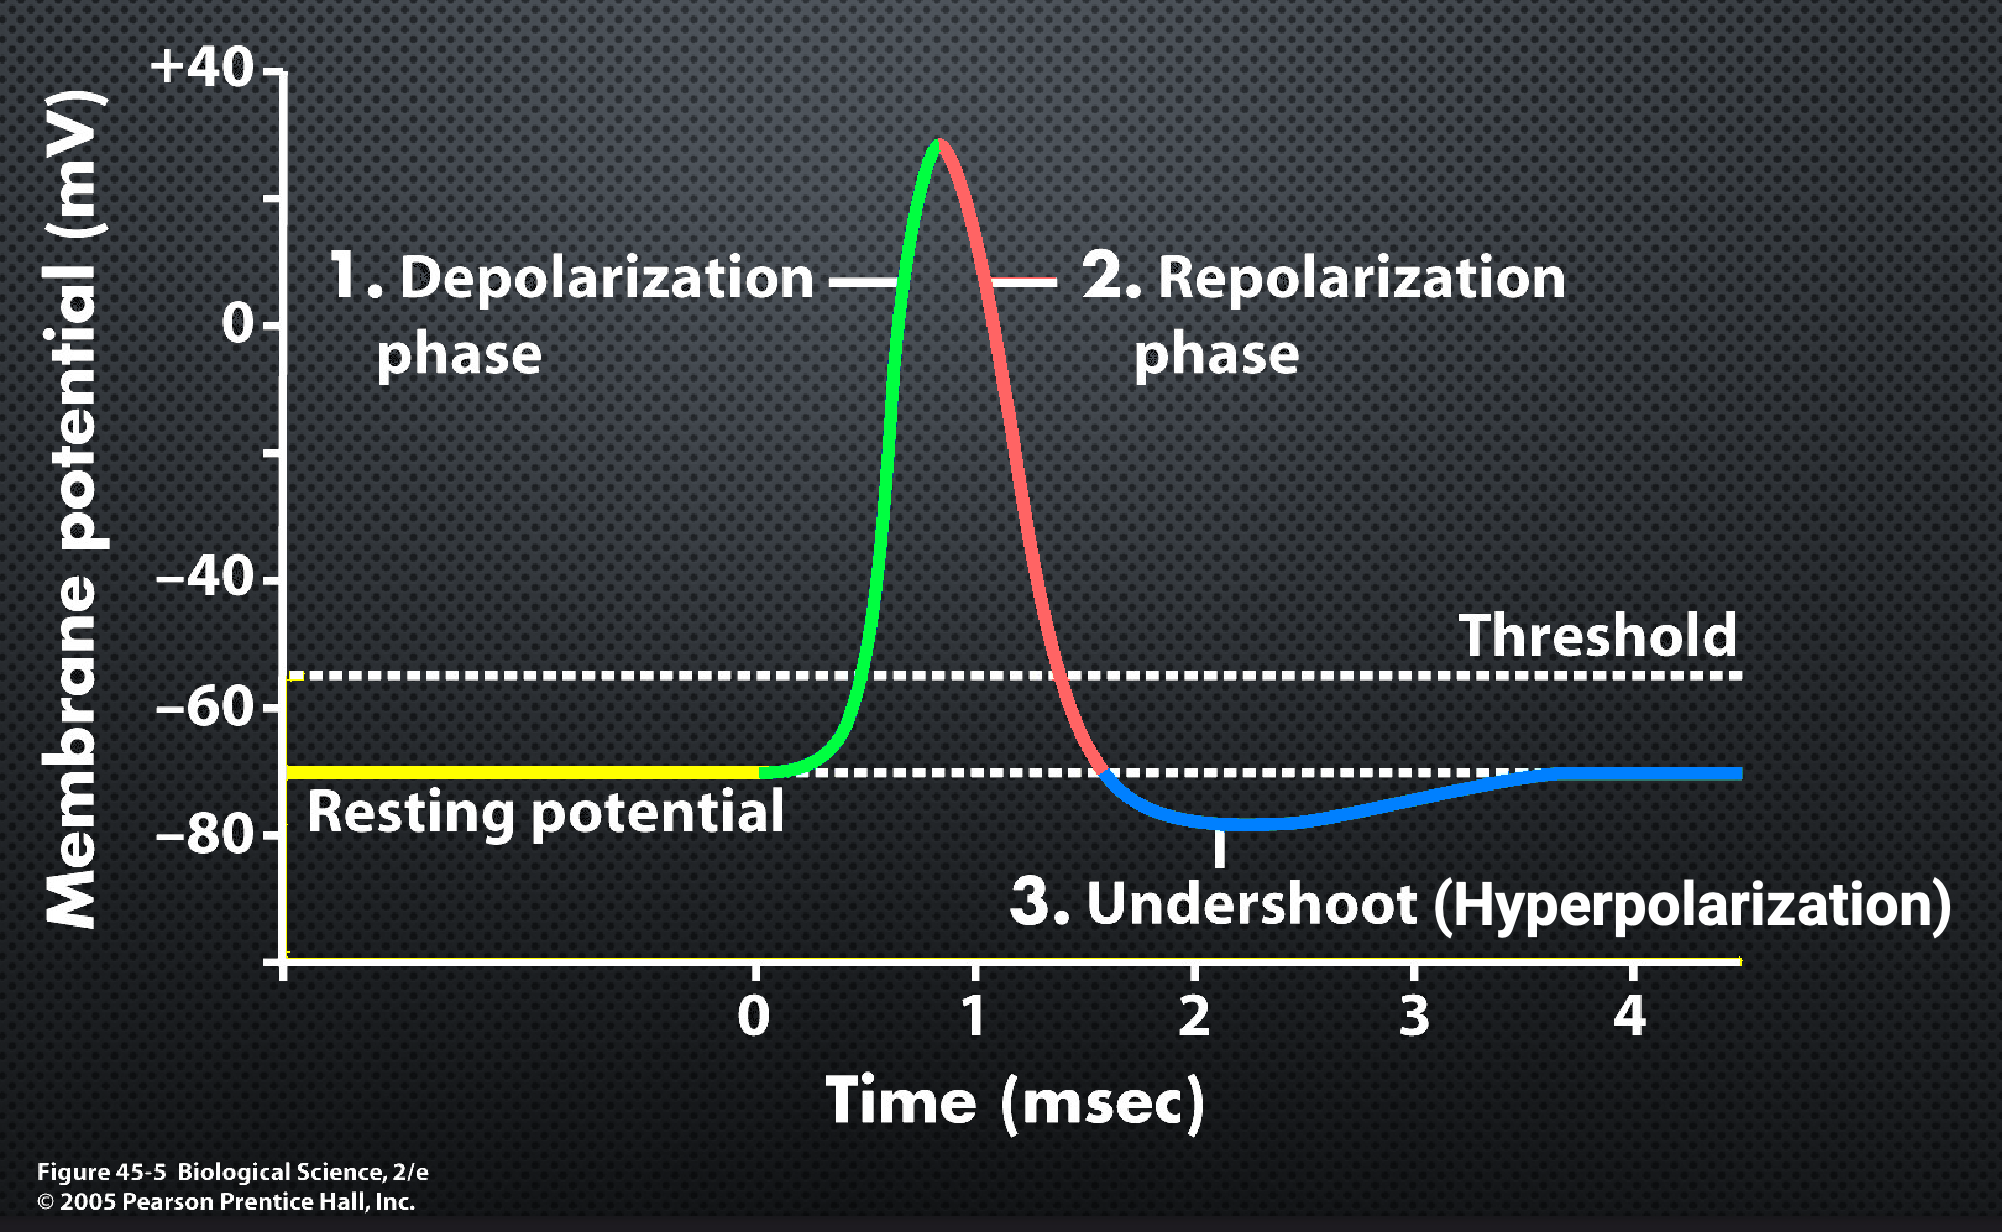
\includegraphics[width=0.5\textwidth]{neuron-spike.png}
\caption{Neuron Spike}
\end{figure}

\begin{itemize}
\tightlist
\item
  \emph{Resting} at \(-70\si{mV}\)
\item
  \emph{Depolarization phase}: Excitation from input signal reaching an
  artificial threshold resulting in a voltage jump (up to
  \(+40\si{mV}\))
\item
  \emph{Repolarization phase}: Return to resting potential
\item
  \emph{Undershoot (Hyperpolarization)} return to resting.
\end{itemize}

All voltages with respect to outside brainfluid.

This process thakes around \(3\si{ms}\ \left( 333.33\si{Hz} \right)\).
The \emph{Myelin Sheaths} decreases performance and throughput aswell.
This is faster due to thight packing and parallel processing.

The spike is seemingly identical between different neurons (same
Amplitude and timeframe).

\hypertarget{resting-membrane-potential-default-state}{%
\subsubsection{Resting membrane potential (default
state)}\label{resting-membrane-potential-default-state}}

Different ion concentration: more negative inside the neuron than
outside. Measurement in reference to outside. Outside: Mostly
\(\mathit{Na}+\) and \(\textit{Cl}-\). Inside: \(\mathit{K}+\) and
\(\mathit{A}-\). Resting voltage sits at around
\(-65\si{mV} \text{ to } -70\si{mV}\).

\hypertarget{de-polarization}{%
\subsubsection{De-polarization}\label{de-polarization}}

Ions flow through the neuron. Signal excites gates. Gates are
ion-specific and only allow certain kinds of ions. These are
\emph{voltage-gates channels}.

Ions like Sodium (\(\mathit{Na}+\)) enter the neuron resulting in a
positive voltage swing up to \(+40\si{mV}\). Once all Sodium gates are
open the threshold is reached. The gates open with very little voltage.

\hypertarget{hyper-polarization}{%
\subsubsection{Hyper-polarization}\label{hyper-polarization}}

Once the voltage between neuron and outside fluid is positive, the
Sodium gates close (as they're voltage controlled). Respectively the
Potassium (\(\mathit{K}+\)) gates open. Positive charge leaves the
neuron making the voltage drop to below the threshold. At resting
potential the Potassium gates close. Due to the delay in closure
undershoot occurs.

\hypertarget{encoding-information}{%
\subsubsection{Encoding Information}\label{encoding-information}}

Information is seemingly encoded in timeing between pulses. Amplitudes
and Durations of spikes are too simmilar between spikes.

\hypertarget{artifical-neruons}{%
\subsection{Artifical Neruons}\label{artifical-neruons}}

\hypertarget{perceptrons}{%
\subsubsection{Perceptrons}\label{perceptrons}}

A simple neural model.

All dendrites \(u_i\) get weighted \(w_i\) and summed resulting in the
activation \(z\). The summation simulates the \emph{soma} core.
\[z = \sum_{i=1}^{n} \omega_i \cdot u_i\]

The threshold and axiom are simulated by an activation function \(\phi\)
resulting in the \emph{perceptrons'} output \(v\). \[v = \phi(z)\]

Activation functions tend to clamp the output in the range of \(-1\) to
\(1\).

An activation function dictates the output space. A heaviside function
can only output a binary result. Functions with infinite range may
diverge. Sigmoid functions can't overflow however the may saturate. The
computataional cost is quite prohibitive.

\hypertarget{hodgkin-huxley-model}{%
\subsubsection{Hodgkin-Huxley Model}\label{hodgkin-huxley-model}}

\begin{figure} [h]
\centering
    \begin{circuitikz}[]
    \draw (0,0) to [short, o-*] ++(0,1);
    \draw (0,7) to [short, *-o] ++(0,1);
    \draw (-3,7) -- (3,7);
    \draw (-3,1) -- (3,1);
    \draw (-3, 1) to[C] ++(0,6);
    \draw (-1, 1) to[C, *-] ++(0,3) to[R, -*] ++(0,3);
    \draw (1, 1) to[C, *-] ++(0,3) to[R, -*] ++(0,3);
    \draw (3, 1) to[C,] ++(0,3) to[R,] ++(0,3);
    \end{circuitikz}
\caption{}
\end{figure}

\end{document}
